
\chapter{Menu Scalars}\label{scalars_chapter}
\minitoc 

Numbers (= scalar values) can be associated to each vertex of a given surface, and are referred to as "scalar arrays". 
As stated earlier, a given unselected surface can be colored using the currently active scalar array, if that surface contains that scalar array (see also Fig. \ref{4color_modes}-B p.\pageref{4color_modes}). To do so, the array display mode button must be pressed (
\includegraphics[scale=0.7]{images/04/show_color_scale.png}), and a scalar array must be selected as the currently active scalar (ex:
\includegraphics[scale=0.5]{images/04/scalarcombo_scalar.png}). The way scalar arrays are translated into colors can be set up using color "Lookup tables" (LUT), also referred to as color transfer functions. The "Scalar rendering options" window can be opened by clicking on "
\includegraphics[scale=0.7]{images/04/color_scale_edit.png}" (see also Fig. \ref{scalar_rendering_options_window}).

\section{Open scalar rendering option window}
\section{Compute distance from camera for each selected surface}
\section{Compute thickness within each selected surface}
\section{Compute thickness between two surfaces}
\section{Compute curvature for each selected surface}
\section{Compute complexity for each selected surface}
\section{Smooth active scalars for each selected surface}


\noindent
\begin{minipage}{0.5\textwidth}
Scalar values can be associated to each vertex. Scalar values can be displayed when scalar display mode is active. To activate/deactivate scalar display mode, click on ``
\includegraphics[scale=0.7]{images/pixmap/show_color_scale.png}".
When active, the rainbow color scale (see Fig. \ref{rainbow_color_scale}) shows up in the
bottom-right part of the 3D rendering window.
\end{minipage}    
\begin{minipage}{0.5\textwidth}\centering
  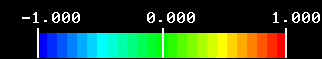
\includegraphics[scale=0.5]{images/Scalars_renreding/color_scale.png}
 \captionof{figure}{Rainbow color scale, showing a
``min" range display value of -1, a
``max" range display value of 1, and a
middle range display value of 0.
}
\label{rainbow_color_scale}
 \end{minipage} 
\noindent


\section{Show scalar rendering options window.}


\begin{figure}
  \centering
  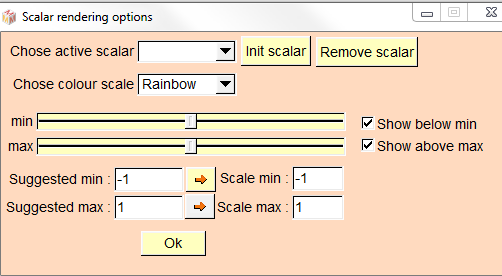
\includegraphics[scale=0.5]{images/Scalars_renreding/color_scale_rendering_window.png}
\caption{Scalar rendering options window}	
\label{Scalar_rendering_options_window}
 \end{figure}


Displayed scalars and scalar associated
color scales can aslo be onpened by
clicking on ``
\includegraphics[scale=0.7]{images/pixmap/edit_color_scale.png}" (see Fig. \ref{Scalar_rendering_options_window}).\\
\noindent
\textbf{\underline{Available controls:}}\\
\textit{Chose active scalar}: please chose among
the available scalars (see below for further
information).\\
\textit{Chose color scale}: please chose among
the available color scales (see below for
further information).\\


\textit{Init scalar}: set current active scalar values to ``0" for all selected objects.
Remove scalar : removes active scalar for all selected objects. This option is useful if you plan to save surfaces in the .vtk format and do not want ISE-MeshTools to save associated scalar values (this will save some disk space).\\
\textit{min}: changes the minimal value of the active color scale.\\
\textit{max}: changes the maximal value of the active color scale.\\
\textit{Show below min}: if active, all vertices with an associated active scalar value below ``min" will be drawn using the color situated at the leftmost part of the active color scale. If not, these vertices will be transparent.\\
\textit{Show below max}: if active, all vertices with an associated active scalar value above ``max" will be drawn using the color situated at the rightmost part of the active color scale.\\
\textit{Suggested min}: suggested ``min" range display value. This value is computed in order to use the
color scale at its best.\\
\textit{Suggested max}: suggested ``max" range display value. This value is computed in order to use the
color scale at its best.\\
``
\includegraphics[scale=0.7]{images/pixmap/s_right_132.png}": Set min/max to suggested min/max, respectively.\\
\textit{Scale min}: current ``min" range display value.\\
\textit{Scale max}: current ``max" range display value.
\textit{Ok}: applies changes.


\section{Scalars: distance from camera (Depth).}
\noindent
\begin{minipage}{0.5\textwidth}
Computes distance from camera for all vertices of
all selected objects. This option may offer a better
perception of the 3D structure of an object on a
2D screen representation.
\end{minipage}    
\begin{minipage}{0.5\textwidth}\centering
  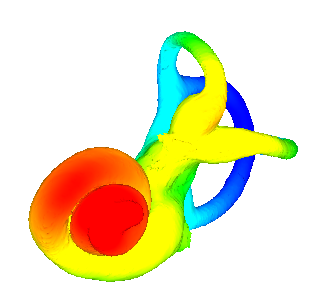
\includegraphics[scale=0.5]{images/Scalars_renreding/Depth.png}
 \captionof{figure}{Example of 3D rendering of ``Depth" scalars.
Scalar mode is active, the rainbow color scale
is used.
}
\label{depth_scalar}
 \end{minipage} 
\noindent



\section{Scalars : compute vertice curvature.}

\noindent
\begin{minipage}{0.5\textwidth}
vtkCurvatures filter is implied in this option.\\
vtkCurvatures filter offers 4 ways to compute surface's
curvature at each vertex (see Fig. \ref{curvatures}):\\
- Principal maximal curvature\\
- Principal minimal curvature\\
- Gaussian curvature\\
- Mean curvature.\\
See vtkCurvatures' documentation for further details.

\end{minipage}    
\begin{minipage}{0.5\textwidth}\centering
  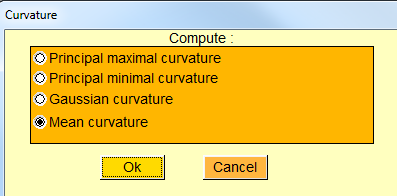
\includegraphics[scale=0.5]{images/Scalars_renreding/Curvature_window.png}
 \captionof{figure}{Curvature window}
\label{curvature_window}
 \end{minipage} 
\noindent

\begin{figure}
  \centering
  \includegraphics[scale=0.3]{images/Scalars_renreding/Curvatures.pdf} 
	\caption{
Examples of 3D rendering of ``Curvature" scalars. Scalar mode is active, the rainbow color scale is used. Specimen : enamel dentine junction (EDJ) of the second superior molar of a juvenile medieval human from Sains-en-Gohelle (France). Specimen number : SP07. Image credit: Mona Le Luyer (PACEA, Bordeaux).}
\label{curvatures}
 
\end{figure}

\section{Scalars: compute thickness.}
\noindent
\begin{minipage}{0.5\textwidth}
Thickness within an object (see Fig. \ref{thickness}) is defined the following way: for a
given vertex, the minimal distance between this vertex and other
vertices in the direction opposite to that of the surface's normal
is computed. In order to minimize computation time, a maximal
distance (Maximal thickness (mm) ) is asked to the user, in order
to reduce the amount of vertices investigated at a given location.
\end{minipage}    
\begin{minipage}{0.5\textwidth}\centering
  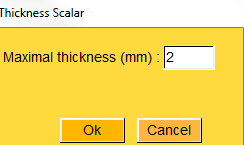
\includegraphics[scale=0.5]{images/Scalars_renreding/Thickness_window.png}
 \captionof{figure}{Thickness scalar window}
\label{thickness_window}
 \end{minipage} 
\noindent





\section{Scalars: compute thickness between two objects.}
\noindent
\begin{minipage}{0.5\textwidth}
Thickness between tow objects is defined the following way (see Fig. \ref{thickness2}):
for a given vertex of the impacted object, the minimal distance
between this vertex and other vertices of the observed surface in
the direction opposite to that of the impacted surface's normal
is computed. Again, in order to minimize computation time, a
maximal distance (Maximal thickness (mm) ) is asked to the user,
in order to reduce the amount of vertices investigated at a given
location. Only selected surfaces appear in the impacted object
and observed object lists.
\end{minipage}    
\begin{minipage}{0.5\textwidth}\centering
  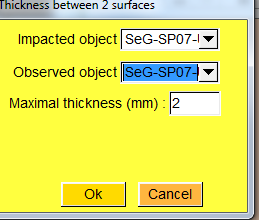
\includegraphics[scale=0.5]{images/Scalars_renreding/Thickness_window2.png}
 \captionof{figure}{Thickness between 2 surfaces window}
\label{thickness_window2}
 \end{minipage} 
\noindent


\noindent
\begin{minipage}{0.5\textwidth}\centering
 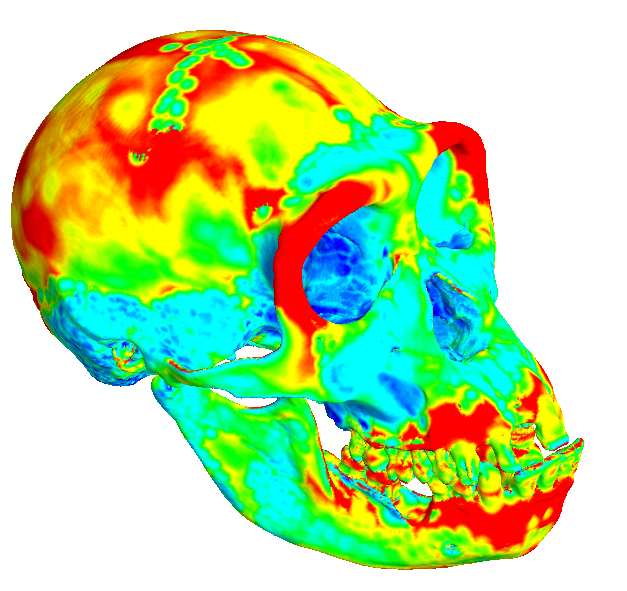
\includegraphics[scale=0.3]{images/Scalars_renreding/Thickness2.png}
 \captionof{figure}{Example of 3D rendering of ``Thickness" of the
3D model ot the type specimen of \textit{Pan paniscus}
(downloadable on \href{http://www.metafro.be/primates/panpaniscustype}{Metafro.be}). Scalar mode is active,
the rainbow color scale is used.
Thickness between 2 surfaces
window}
\label{thickness}

\end{minipage}    
\begin{minipage}{0.5\textwidth}\centering
  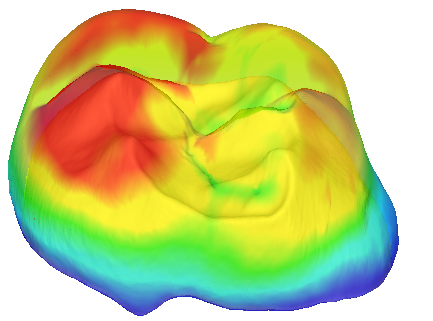
\includegraphics[scale=0.5]{images/Scalars_renreding/thickness_.png}
 \captionof{figure}{Example of 3D rendering of ``Thickness" between
two objects' scalars. Scalar mode is active,
the rainbow color scale is used. Impacted
object : enamel surface of SP07 specimen (see
above for details). Observed object : enameldentine
junction's surface (EDJ) of SP07 specimen.}
\label{thickness2}
 \end{minipage} 
\noindent





\section{Smooth active scalars (Gaussian blur).}
Active scalars are ``smoothed" the following way : for each vertex, a new scalar value is computed as
the mean of the scalar values of all neighbouring vertices (see Fig. \ref{smoothing_scalars}).
\begin{figure}
  \centering
  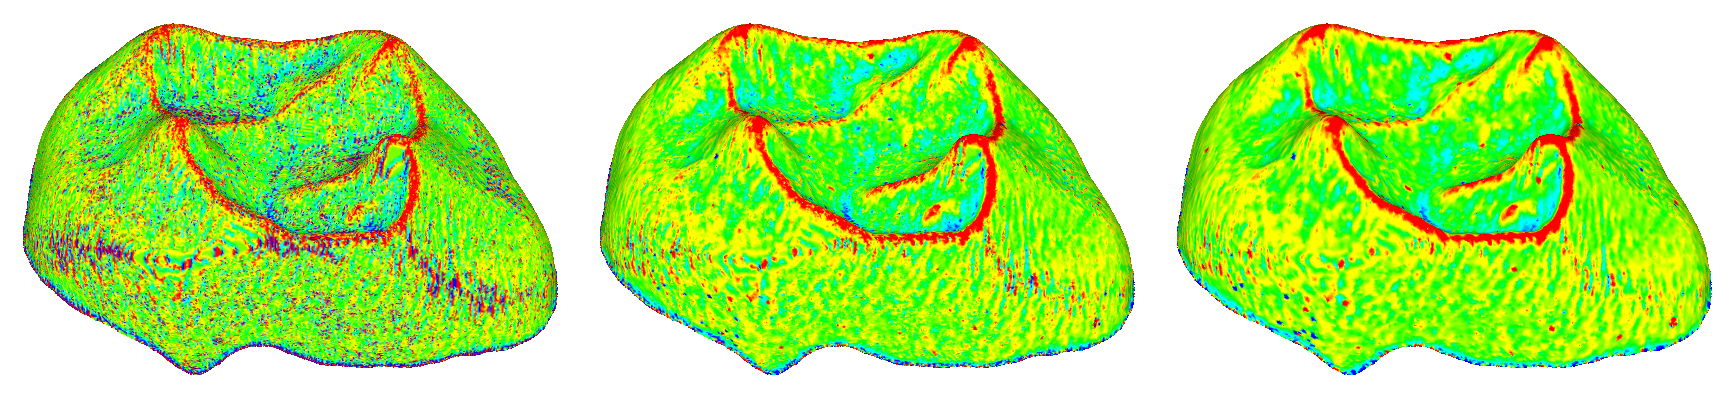
\includegraphics[scale=0.25]{images/Scalars_renreding/Smooth_012.png} 
	\caption{Smoothing scalars. Examples of 3D rendering of ``Mean Curvature" scalars. Scalar mode is active, the rainbow color scale is used. Left : ``raw" mean curvature. Middle : mean curvature scalars smoothed once. Right : mean curvature scalars smoothed twice. Specimen: EDJ of SP07 specimen.}
\label{smoothing_scalars}
 
\end{figure}


\section{Init RGB.}
Whenever colors are associated to vertices in .PLY of .VTK files (this can be achieved for instance by painting on meshes with Meshlab or by transferring textures obtained by laser scanning to the vertices), ISE-MeshTools stores this ``initial RGB" color information inside a dedicated scalar (called ``Init\_RGB"). See for instance Fig. \ref{rgb_scalar}.
\\Note: you have to select a Mesh in order to activate this option.

\begin{figure}
  \centering
  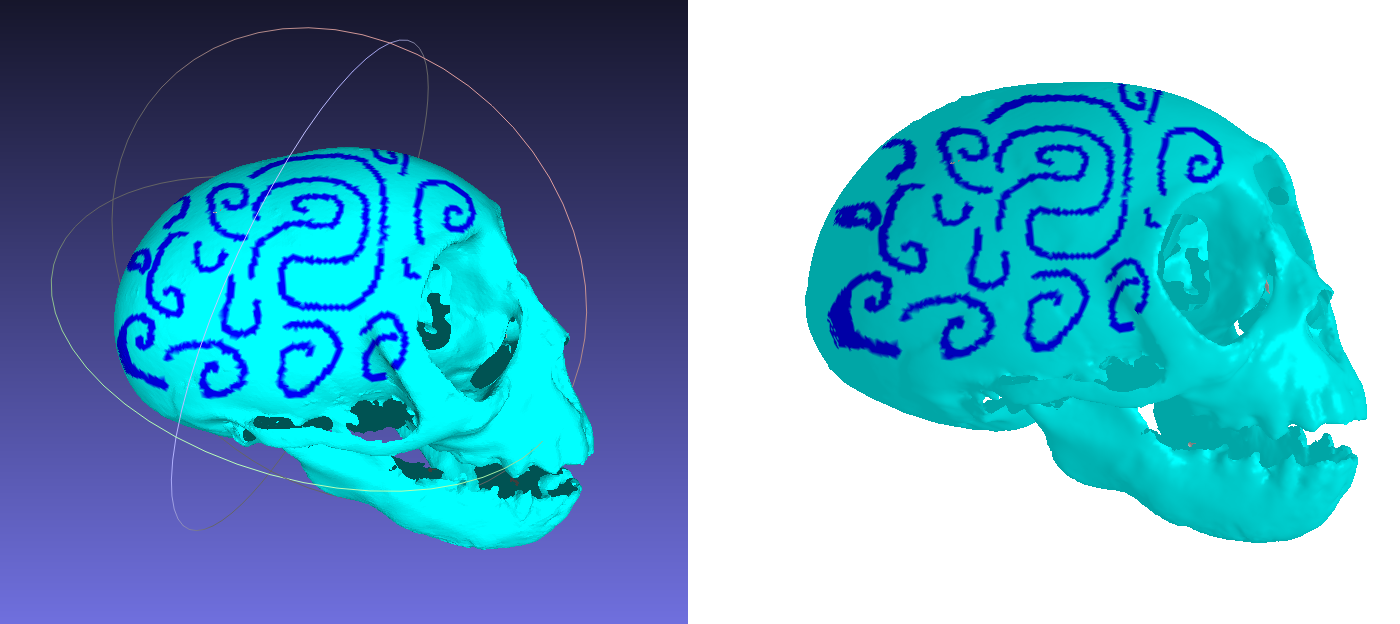
\includegraphics[scale=0.3]{images/Scalars_renreding/init_rgb.png} 
	\caption{Initial RGB Scalar. Left: a mesh is painted using Meshlab. Right: the same mesh opened with ISE-MeshTools using the ``Init RGB" option.}
\label{rgb_scalar}
 
\end{figure}

\section{Saving and loading scalars.}
Computed scalars can be saved inside the .vtk surface files. In order to access scalar values into other software (such as a text editor), save the .vtk files in ASCII format. Saved scalars can be reloaded into ISE-MeshTools. Saving surfaces into .vtk format provides an efficient means to store and exchange
computed scalars.
